\bookchapter{第四十九章：搭建開發環境——Android Studio 同第一個項目}

\chapterintro{工欲善其事，必先利其器。呢一章我哋將個「廚房」搭好：裝好 Android Studio、行通模擬器、開人生第一個安卓項目，再將工程結構拆開睇個明明白白。裝好環境之後，你會第一次見到自己寫嘅程式碼變成一個篤得到嘅掣——呢一刻，好多人會記一世。}

\booksection{一、安裝 Android Studio}

Android Studio 係谷歌官方嘅集成開發環境（IDE），免費，功能全家桶：寫程式碼、睇介面預覽、除錯、打包全部都喺入面。安裝四步：

\begin{enumerate}
  \item 打開官網 developer.android.com/studio，下載最新穩定版（2026 年 8 月係 Narwhal 之後嘅版本，Windows/Mac/Linux 都有）；
  \item 行安裝包，一路撳「下一步」——安裝精靈會自動帶埋 Android SDK 同模擬器組件；
  \item 第一次啟動嗰陣跟提示下載 SDK 組件（用預設勾選就好，可能要幾分鐘同幾個 GB 嘅空間）；
  \item 搞掂之後你會見到歡迎頁——恭喜，個「廚房」搭好喇。
\end{enumerate}

\begin{tcbwarn}{注意：硬件要求心入面有數}
Android Studio 係個「食記憶體」嘅傢伙：建議 16GB 記憶體起步（8GB 都行到，但係一開模擬器就會比較卡）、磁碟預留 20GB 以上、CPU 要支援虛擬化（喺 BIOS 入面開 VT-x/AMD-V）。如果部電腦真係舊，可以用「真機除錯」代替模擬器（本章第四節會講），體驗反而更加暢順。

\end{tcbwarn}

\booksection{二、開你嘅第一個項目}

喺歡迎頁撳 New Project，揀 Empty Activity 模板（最乾淨嘅新手模板），跟住填三樣嘢：

\begin{center}
\begin{tabularx}{\linewidth}{|X|X|X|}
\hline
\textbf{配置項} & \textbf{填乜嘢} & \textbf{說明} \tabularnewline
\hline
Name & My First App & App 名字，會顯示喺手機桌面上面 \tabularnewline
Package name & com.example.myfirstapp & 全球唯一標識，慣常做法係「域名反寫」，先用預設 \tabularnewline
Minimum SDK & API 26（Android 8.0） & 最低支援版本，覆蓋 95\% 以上設備 \tabularnewline
\hline
\end{tabularx}
\end{center}

\begin{center}\small\color{gray}開項目要填嘅三樣嘢\end{center}

撳完 Finish 之後，Android Studio 會用 Gradle 自動下載依賴、構建項目（第一次要等幾分鐘，之後每次會快好多）。構建完成之後，你就有一個行到嘅 App——雖然佢仲淨係識顯示一行「Hello Android!」。

\begin{tcbinfo}{小貼士：包名嘅門道}
包名（package name）就好似 App 嘅「身份證號碼」，全球唔可以重複，上咗架之後就唔可以改。個人練習用 com.example.xxx 就得；正式產品要換成你自己嘅域名反寫（例如 com.你個名.應用名）。唔好攞 com.example 嚟上架——商店會拒收。

\end{tcbinfo}

\booksection{三、行起上嚟：模擬器同真機}

程式碼寫好咗，就要搵部「手機」嚟行。你有兩個選擇：

\booksubsection{模擬器（Emulator）}

模擬器係喺電腦入面虛擬出一部安卓手機。喺 Android Studio 入面打開 Device Manager Create Device，揀一部設備（推薦 Pixel 系列） 揀一個系統映像（帶 Google APIs 嗰種） 下載 啟動。跟住撳工具列嘅綠色三角 Run，幾秒之後，「手機」螢幕上面就會出現你個 App。

\booksubsection{真機除錯（更加推薦）}

真機永遠係最真實嘅測試環境——滑動手感、真網絡、真感應器，模擬器都比唔上。安卓真機除錯好簡單：

\begin{enumerate}
  \item 手機上面打開 [設定] [關於手機]，連續篤「版本號」7 次，開啟「開發者選項」；
  \item 喺 [開發者選項] 入面打開 USB 除錯；
  \item 用傳輸線駁電腦，手機彈窗揀「允許 USB 除錯」；
  \item 返去 Android Studio，工具列嘅設備下拉清單入面就會出現你部手機，撳 Run。
\end{enumerate}

\textbf{避坑提醒：USB 除錯唔好長開}\par

USB 除錯等於畀部電腦開咗個「後門」。喺公眾場合充電、駁去唔信任嘅電腦嗰陣，一定要閂咗 USB 除錯，防止其他人透過佢讀取你嘅資料。平時開發用完就閂，養成習慣。

\booksection{四、工程結構拆解：每個檔案係做乜嘢嘅}

第一次打開項目，左邊嘅檔案樹可能會令你頭暈。唔使慌，日常開發你 90\% 嘅時間淨係會同下面呢幾個打交道：

\begin{center}
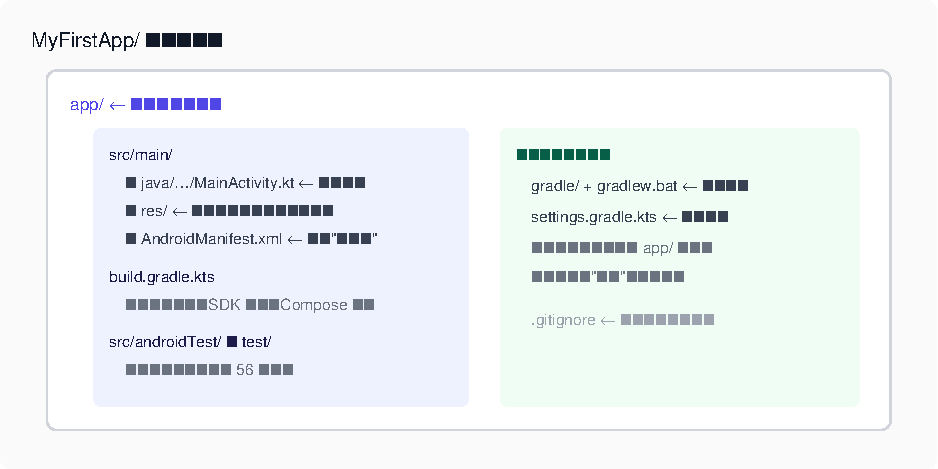
\includegraphics[width=0.92\linewidth]{figures/fig-di-si-shi-jiu-zhang-1}
\\[2pt]\small 圖 2：新手必識嘅工程結構（口訣：淨係掂 app/ 目錄）
\end{center}

\begin{itemize}
  \item MainActivity.kt：App 嘅「大門」。用戶篤開個圖示，第一個被喚醒嘅就係佢。而家嘅模板入面佢負責顯示「Hello Android!」。
  \item AndroidManifest.xml：App 嘅「戶口簿」——聲明呢個 App 叫乜嘢名、圖示係邊個、有邊啲頁面、要用邊啲權限（相機、定位等等）。
  \item res/ 目錄：資源倉庫，存圖片、圖示、字串、顏色。將文字放喺資源檔而唔係寫死喺程式碼入面，係安卓開發嘅好習慣（換語言、換主題都方便）。
  \item build.gradle.kts：構建配方——聲明最低支援版本、依賴邊啲函式庫（例如 Compose）。
\end{itemize}

\booksection{五、小試牛刀：將「Hello」換成你個名}

打開 MainActivity.kt，你會見到 Compose 模板生成嘅程式碼。搵到 Text(“Hello Android!”) 呢一行，將引號入面嘅字換成你個名，例如 Text(“你好，張三！呢個係我嘅第一個App”)，跟住撳 Ctrl+R（Mac 係 Cmd+R）重新運行。幾秒之後，模擬器上面就會顯示你個名。

\begin{lstlisting}[language=Kotlin]
setContent {
    MyFirstAppTheme {
        Surface(modifier = Modifier.fillMaxSize()) {
            // v 把呢度改成你自己嘅文字
            Text("你好，張三！呢個係我第一個App")
        }
    }
}
\end{lstlisting}

恭喜，你已經完成咗一次完整嘅「改程式碼 編譯 安裝 運行」循環。呢個循環，就係將嚟每一日嘅開發日常。趁熱打鐵，試嚇再改啲其他嘢：將字號調大、轉個顏色——下一章我哋就會學到呢啲「魔法」係點樣嚟嘅。

\booksection{六、常見報錯急救：新手頭兩個禮拜嘅「急症室」}

搭環境同第一次構建嘅階段，你好大機會遇到下面三種報錯。唔使慌，全部都有解藥：

\begin{center}
\begin{tabularx}{\linewidth}{|X|X|X|}
\hline
\textbf{報錯現象} & \textbf{常見原因} & \textbf{解藥} \tabularnewline
\hline
Gradle sync failed / 依賴下載慢 & 網絡訪問倉庫唔暢順 & 畀 Gradle 配置國內鏡像倉庫（阿里雲／騰訊雲 maven 鏡像），上網搜「gradle 國內鏡像」跟住改 \tabularnewline
SDK 組件缺失 & 安裝嗰陣跳過咗 SDK 下載 & Settings SDK Manager 補裝缺失嘅平臺同工具 \tabularnewline
模擬器啟動失敗 / 黑屏 & 虛擬化未開啟、映像損壞 & 喺 BIOS 開 VT-x/AMD-V；刪咗模擬器再建過；或者直接用真機除錯 \tabularnewline
\hline
\end{tabularx}
\end{center}

\begin{center}\small\color{gray}新手環境報錯急救表\end{center}

\begin{tcbinfo}{小貼士：搜報錯嘅方法論}
報錯資訊第一行係最有價值嘅——將佢原封不動複製入搜尋引擎，加埋「android studio」呢個關鍵詞。唔好搜「我裝唔到環境點算好」呢啲籠統問題，要搜「Gradle sync failed: Could not resolve com.android.tools.build」呢啲具體錯誤。精確嘅問題，先至有精確嘅答案。

\end{tcbinfo}

\begin{tcbpractice}{嚟動手：完成你嘅「開發儀式感」清單}
(1) 裝好 Android Studio 並且行通模擬器；(2) 用真機行一次自己個 App 並且截圖留念；(3) 將 Hello 嗰句字改成你個名；(4) 將項目壓縮存個檔。做完呢四步，你就可以喺朋友圈宣佈：我都係安卓開發者喇（有圖為證）。

\end{tcbpractice}

\begin{tcbsummary}{本章小結}
\begin{itemize}
  \item Android Studio = 官方免費 IDE；建議 16GB 記憶體 + 20GB 磁碟 + 開虛擬化
  \item 新建項目三要素：名字、包名（全球唯一，com.example 唔好攞去上架）、最低 SDK（API 26 起）
  \item 兩種運行方式：模擬器（電腦入面虛擬手機）同真機（開 USB 除錯，用完記得閂）
  \item 工程口訣：淨係掂 app/ 目錄——MainActivity.kt 係大門，Manifest 係戶口簿，res/ 係資源倉庫
  \item 開發日常 = 改程式碼 Run 睇效果，循環往復
\end{itemize}

\end{tcbsummary}
